\documentclass[journal]{IEEEtran}

\usepackage{mathtools}
\usepackage{amsmath,amssymb,amsthm}
\usepackage{graphicx}
\usepackage{caption}
\usepackage{subcaption}
\usepackage{hyperref}
\usepackage{float}
\usepackage{wrapfig}

\graphicspath{{assets/}}

\newtheorem{theorem}{Theorem}[section]
\newtheorem{remark}{Remark}[section]

\begin{document}

\title{Twice-around a Shortest-path Tree Significantly Increases the Solution Cost}

\author{Prof. Dr. Alexandre L. M. ~Levada,
	Lucas O. ~David
\thanks{Alexandre L. M. Levada and Lucas O. David are with Universidade Federal de Sao Carlos.}%
%\thanks{Manuscript received April 19, 2005; revised January 11, 2007.}%
}

\markboth{\today}%
{Shell \MakeLowercase{\textit{et al.}}: icgraphlucas}

\maketitle

\begin{abstract}

In the Graph Theory field, one of the most important problems is the Traveling Salesman Problem. Many algorithms have been developed to solve or approximate this problem, with one of them being the Twice-around Algorithm. This paper describes the behavior of the Twice-around algorithm when it has as input a shortest-path tree instead of its default minimum spanning tree. Through empirical experimentation, we discovered that the modified Twice-around consistently presented poor solutions compared to the original algorithm.

\end{abstract}

\begin{IEEEkeywords}
	Graph Theory, Traveling Salesman Problem, Twice-around.
\end{IEEEkeywords}

\section{Introduction}

In our world, it is possible to model a considerable set of problems using the Traveling Salesman Problem (TSP), making it one of the most popular existing algorithms. The study of methods that solve or satisfactorily approximate a solution is of great importance, as it would imply great development in many different areas of knowledge that depend on computational feasibility.

Currently, many different approaches are employed to solve the TSP. While some will seek the optimal answer through a smart (but possibly exhaustive) search, as Branch-and-bound or the Held-Karp algorithm, others will base themselves on heuristics to find a candidate-solution with reasonable cost (e.g. Lin-Kernighan or ant community optimization \cite{soricone}).

This project aim to develop the basic algorithms involved (e.g. Dijkstra's, Prim's, Depth-First search, Twice-around), as well as an environment capable of creating or collecting instances of the problem from a database and running test between the original and the modified Twice-around algorithms. All results and necessary implementations can be found on this code repository: \href{https://github.com/lucasdavid/tsp}{tsp}.

\section{The Traveling Salesman Problem}
\label{s:tsp}

Let $G=(X, E)$ be the k-complete symmetric weighted graph, where $X$ is a set of cities and $E$ the set of edge that represents the distances between different cities. The Traveling Salesman Problem (TSP) has as goal find the Hamiltonian Circuit such that the sum of edges' weights is minimum.

\section{The Twice-around Algorithm}

The Twice-around algorithm is an heuristic broadly employed when solving the TSP. 

Let $G$ be defined as in section \ref{s:tsp}, the twice-around algorithm will transverse a minimum spanning tree extracted from $G$ using a search algorithm such as \textbf{Depth-First Search} while records the vertices visited. It will then proceed to remove the repetitions in the recorded sequence, expect for last vertice \cite{nilsson}.

\subsection{Twice-around Execution Example}

Let $G$ be the graph defined in figure \ref{fig:ex-ta-1}, $A$ the starting node and $M$ the minimum spanning tree extracted from $G$.

\begin{figure}[H]
	\begin{subfigure}{.5\linewidth}
		\centering
		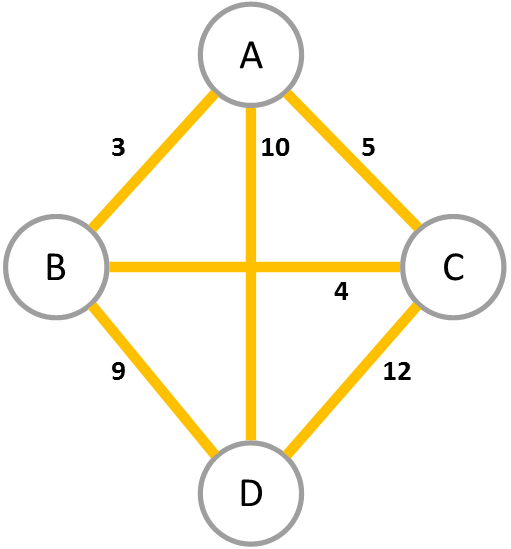
\includegraphics[width=.5\linewidth]{ex-ta-1}
		\caption{The graph $G$.}
		\label{fig:ex-ta-1}
	\end{subfigure}%
	\begin{subfigure}{.5\linewidth}
		\centering
		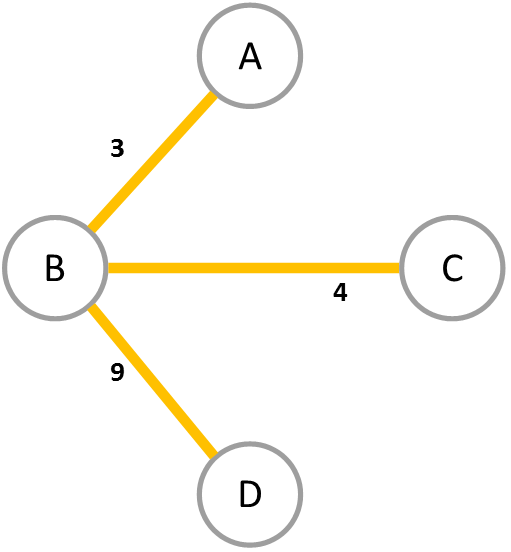
\includegraphics[width=.5\linewidth]{ex-ta-2}
		\caption{The MST $M$.}
		\label{fig:em}
	\end{subfigure}
\end{figure}

$M$ will be transversed and the visiting sequence $L_1 = (A, B, D, B, C, B, A)$ will be recorded. Finally, the repeated vertices are removed. This elimination process can be informally interpreted as ``taking shortcuts". The following figure illustrates how removing the first repetition of $B$ from $L_1$ will link the vertices $C$ and $D$.
\begin{figure}[H]
	\centering
	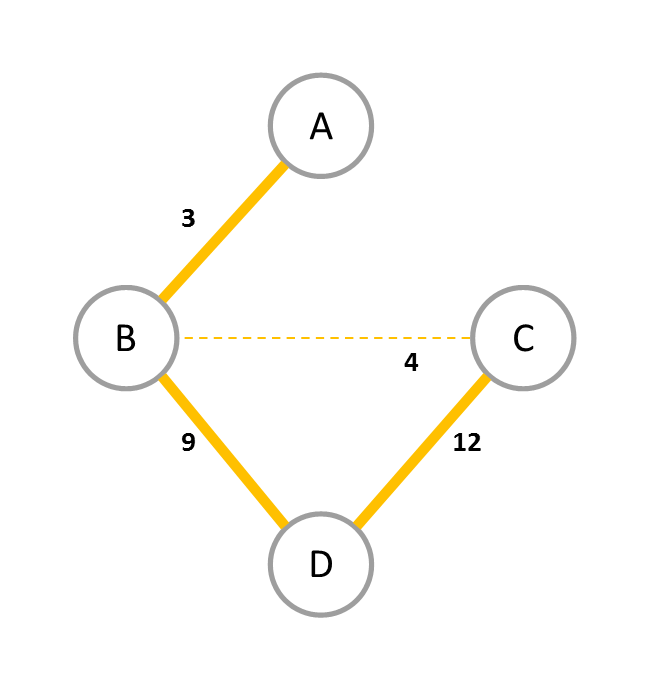
\includegraphics[width=.4\linewidth]{ex-ta-4}
	\label{fig:exta4}
	\caption{MST $M$ with the first $B$ repetiton removed.}
\end{figure}

By eliminating all the repetitions, the algorithm will result in a Hamiltonian circuit candidate $L=(A, B, D, C, A)$ with cost $c_L = 100$:
\begin{figure}[H]
	\centering
	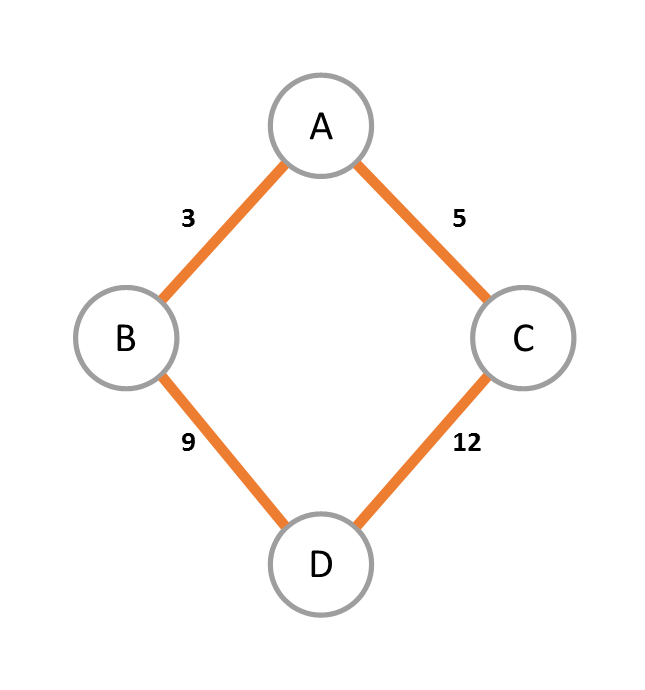
\includegraphics[width=.4\linewidth]{ex-ta-3}
	\label{fig:exta3}
	\caption{The Hamiltonian circuit candidate $L$.}
\end{figure}

\begin{theorem}
	$c_L \le 2 c_{L^\star}$, where $c_P$ is the cost of walking on a circuit $P$, $L$ is the Hamiltonian circuit candidate found and $c_{L^\star}$ is the optimal Hamiltonian circuit.
\end{theorem}
\begin{proof}
	Let $T$ be the spanning tree resulted from removing any edge from $L^\star$ and $M$ be the minimum spanning tree.
	\begin{align*}
	c_{L^\star}   > c_T \ge c_M \iff
	2c_{L^\star} > 2c_M
	\end{align*}
	
	The triangular inequality $\delta_{uv} \le \delta_{uw} + \delta_{wv}, \forall (u, v, w) \in V^3$ holds, as this graph was built over euclidean distances. Therefore,
	\begin{align*}
	2c_M &\ge c_L \\
	\therefore 2c_{L^\star} &> c_L
	\end{align*}
\end{proof}

It's also important to remember that any shortcut done in the MST $m$ will not decrease the sum of costs from the edges of the resulting tree, compared to the sum of edges' costs from the edges in $m$. The example above demonstrates this: the cost of the MST is $3+4+9=16$, whereas the cost of the MST after the firsts shortcut is $5+9+12=26$.

\begin{theorem}
	\label{t:sic}
	Let $m=(V, F)$ be the MST extracted from graph k-complete $G=(V, E)$, $m'$ the path found by shortcutting all branches of $m$, $\delta_{AB}$ the distance between vertices $A$ and $B$, and $c(p)=\sum\delta_{X_iY_i}, p = (V, \{X_iY_i\})$.
	$$c(m') \ge c(m)$$
\end{theorem}
\begin{proof}
	If the MST $m$ contains two edges $AB, AC \in F$ (a branch), leading to two different paths $B...B'$ and $C\dots C'$, $m'' = (V, F-\{AC\}+\{B'C\})$,
    \begin{align*}
    B'C \notin F, AC \in F \implies \delta_{B'C} \ge \delta_{AC} \\
    c(m'') = c(m) - \delta_{AC} + \delta_{B'C} \ge c(m)
    \end{align*}
    
	Now define $m' = (V, L) \mid L = F - \sum {A_iC_i} + \sum {B'_iC_i}$, where $B = \{(A_iB_i, A_iC_i)\}$ is the set with all branches in $m$.
    \begin{align*}
    c(m') &= c(F - \sum \{A_iC_i\} + \sum \{B'_iC_i\}) \\
    &= c(V, F)  - \delta_{A_0C_0} + \delta_{B'_0C_0} \\
    &- \delta_{A_1C_1} + \delta_{B'_1C_1} + \dots \\
    &- \delta_{A_nC_n} + \delta_{B'_nC_n}
    \end{align*}
    But $\delta_{A_iC_i} \le \delta_{B'_iC_i}, \forall i\in [0, |B|)$, which implies
	$$c(m') \ge c(V, F) = c(m)$$B
\end{proof}

\section{Dijkstra's Algorithm}

Differently from the minimum spanning tree, the \textbf{shortest path tree} associated with a graph $G$ and the node $g_0$ express the shortest path between the origin $g_0$ and all the other vertices. In the optimization context, the term ``shortest" refers to the minimum cost required to travel on a path between two vertices.

\begin{theorem}
	\label{t:star}
	Let $G=(V, E)$ be the k-complete graph and $E=\{\delta_{xy}\}, (x, y) \in V^2$ the set of egdes built over euclidean distances. The shortest-path tree with origin $v_0$ is the \textbf{star} $S_{k-1}$ with center $v$.
\end{theorem}
\begin{proof}
	The shortest-path tree $T=(V_1, E_1)$ is such that the path cost between two vertices $u$ and $v$ is minimum. But $\delta_{uv} < \delta_{uw} + \delta_{wv}, \forall (u, v, w) \in V^3, u \ne v \ne w \ne u$ holds in euclidean spaces, so $T = (V_1, \{\delta_{v_0u, \forall u \in V_1}\})$, where $V_1$ is the set of all vertices in the connected cluster in which $v_0$ is placed.
\end{proof}

\section{Experiments}

In order to observe the behavior of the Twice-around algorithm when it has as input a SPT instead of a MST, a analyzer was built. Given a set of S-TSP instances, it will solve all of them with both original and modified Twice-around. Information about the solutions is recorded in each iteration (e.g. costs, elapsed time, best performing algorithm). At the end, a report containing all data collected is issued.

The comparison between the two algorithms was done by three phases, with their respective set of problems.

\subsection{Phase I: Randomly Generated Euclidean Graphs}

Figure \ref{fig:ctreg} illustrates that the modified Twice-around performs worse than the original one in all situations. Additionally, the cost disparity of the solutions quickly increased as the number of vertices grew.

\begin{figure}[H]
	\centering
	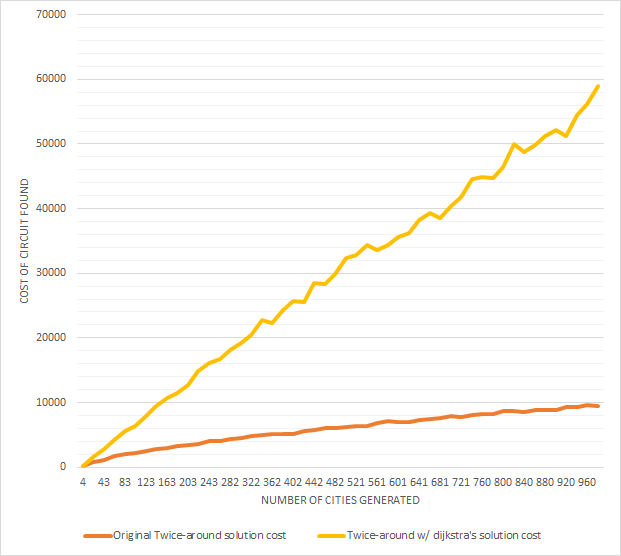
\includegraphics[width=.95\linewidth]{comparison-ta-random-euclidean-graphs}
	\caption{Solutions' costs for random euclidean graphs.}
	\label{fig:ctreg}
\end{figure}

\subsection{Phase II: Real Euclidean Graphs}

Figure \ref{fig:ctrealg} shows the disparity between costs found by both original and modified Twice-around when applied to real instances of the TSP problem. In all four cases, the original Twice-around presented a much better solution than the Twice-around with dijsktra's.

\begin{figure}[H]
	\centering
	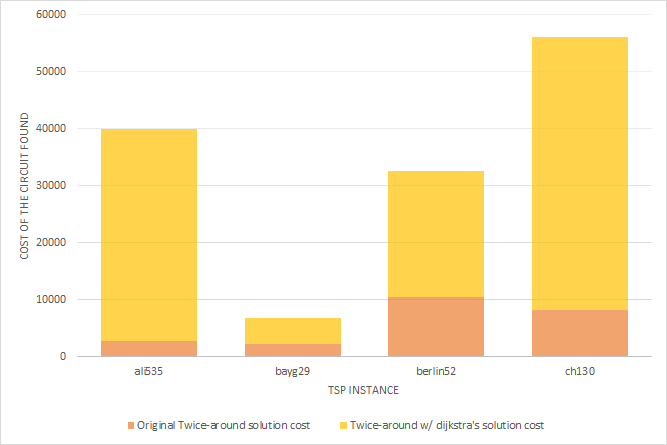
\includegraphics[width=.95\linewidth]{comparison-ta-real-graphs}
	\caption{Solutions' costs for real graphs.}
	\label{fig:ctrealg}
\end{figure}

\subsection{Phase III: Randomly Generated Non-euclidean Graphs}

Figure \ref{fig:ctrg} illustrates that the modified Twice-around consistently presented a worse solution than the original algorithm in non-euclidean random graphs.

\begin{figure}[H]
	\centering
	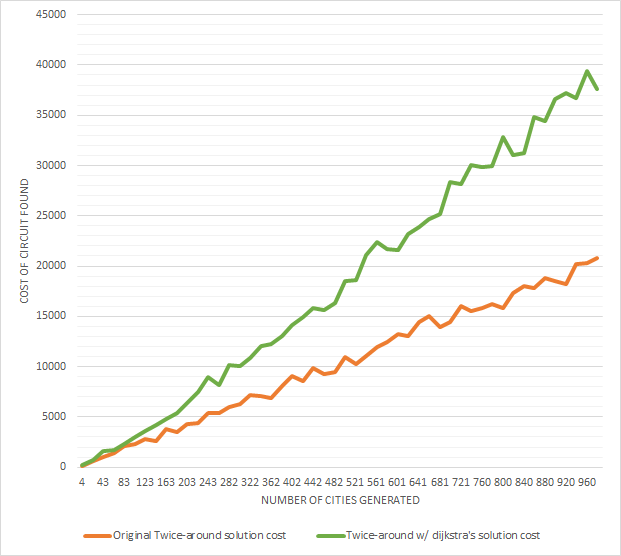
\includegraphics[width=.95\linewidth]{comparison-ta-random-graphs}
	\caption{Solutons's costs for non-euclidean random graphs.}
	\label{fig:ctrg}
\end{figure}

\section{Discussions}

From \ref{t:star}, the shortest path tree found in euclidean graph is a star. The recorded visiting list is then be described as $L_1=(A, B, A, C, A, D, A, E, ..., A)$. With the repetitions removed, the Hamiltonian circuit candidate is $L=(A,B,C, D, E, ..., A)$ with cost $c_L=\sum_{i=0}^{n-2} c(V_i, V_{i+1}) + c(V_{n-1}, V_0)$. Notice that no lower bound can be defined for cost $c_L$. As for shortest-path trees extracted from non-euclidean graphs: although they are not necessarily stars, we observed a tendency of those to have a high number of branches.

If the tree used has few branches, many sub-paths are preserved when building the circuit candidate (few shortcuts are required). In the other hand, as we are required to take many shortcuts in trees with many branches, such as the \textbf{star}, few sub-paths are preserved and the solution cost can drastically change (from \ref{t:sic}, shortcutting increases cost). We believe this to be the main reason for the poor performance of the modified Twice-around.

\section{Conclusion}

This paper presented a modification of the Twice-around algorithm where a SPT was used as input instead of the classic MST. We observed, through empirical experimentation, that this modification performed significantly worse than the original algorithm.

\bibliographystyle{plain}
\bibliography{references}

\end{document}
